\documentclass[a4paper]{article}\usepackage[]{graphicx}\usepackage[]{color}
%% maxwidth is the original width if it is less than linewidth
%% otherwise use linewidth (to make sure the graphics do not exceed the margin)
\makeatletter
\def\maxwidth{ %
  \ifdim\Gin@nat@width>\linewidth
    \linewidth
  \else
    \Gin@nat@width
  \fi
}
\makeatother

\definecolor{fgcolor}{rgb}{0.345, 0.345, 0.345}
\newcommand{\hlnum}[1]{\textcolor[rgb]{0.686,0.059,0.569}{#1}}%
\newcommand{\hlstr}[1]{\textcolor[rgb]{0.192,0.494,0.8}{#1}}%
\newcommand{\hlcom}[1]{\textcolor[rgb]{0.678,0.584,0.686}{\textit{#1}}}%
\newcommand{\hlopt}[1]{\textcolor[rgb]{0,0,0}{#1}}%
\newcommand{\hlstd}[1]{\textcolor[rgb]{0.345,0.345,0.345}{#1}}%
\newcommand{\hlkwa}[1]{\textcolor[rgb]{0.161,0.373,0.58}{\textbf{#1}}}%
\newcommand{\hlkwb}[1]{\textcolor[rgb]{0.69,0.353,0.396}{#1}}%
\newcommand{\hlkwc}[1]{\textcolor[rgb]{0.333,0.667,0.333}{#1}}%
\newcommand{\hlkwd}[1]{\textcolor[rgb]{0.737,0.353,0.396}{\textbf{#1}}}%

\usepackage{framed}
\makeatletter
\newenvironment{kframe}{%
 \def\at@end@of@kframe{}%
 \ifinner\ifhmode%
  \def\at@end@of@kframe{\end{minipage}}%
  \begin{minipage}{\columnwidth}%
 \fi\fi%
 \def\FrameCommand##1{\hskip\@totalleftmargin \hskip-\fboxsep
 \colorbox{shadecolor}{##1}\hskip-\fboxsep
     % There is no \\@totalrightmargin, so:
     \hskip-\linewidth \hskip-\@totalleftmargin \hskip\columnwidth}%
 \MakeFramed {\advance\hsize-\width
   \@totalleftmargin\z@ \linewidth\hsize
   \@setminipage}}%
 {\par\unskip\endMakeFramed%
 \at@end@of@kframe}
\makeatother

\definecolor{shadecolor}{rgb}{.97, .97, .97}
\definecolor{messagecolor}{rgb}{0, 0, 0}
\definecolor{warningcolor}{rgb}{1, 0, 1}
\definecolor{errorcolor}{rgb}{1, 0, 0}
\newenvironment{knitrout}{}{} % an empty environment to be redefined in TeX

\usepackage{alltt}
\usepackage{a4wide}
\usepackage{amsmath, amsfonts, amssymb}
\usepackage{color}
%\usepackage{natbib}

\newcommand{\nn}{\noindent}
\IfFileExists{upquote.sty}{\usepackage{upquote}}{}
\begin{document}



\section*{Running a simple simulation \hfill \normalsize{\textnormal{Jack Kuipers, \today}}}

\nn For this example we simulate data from a DAG with $n=5$ nodes and score with the BGe score.  This code creates the graphs in the main paper.

\begin{knitrout}
\definecolor{shadecolor}{rgb}{0.969, 0.969, 0.969}\color{fgcolor}\begin{kframe}
\begin{alltt}
\hlstd{n} \hlkwb{<-} \hlnum{5}
\end{alltt}
\end{kframe}
\end{knitrout}

\nn First we load the \texttt{R} files needed to run the MCMC codes
\begin{knitrout}
\definecolor{shadecolor}{rgb}{0.969, 0.969, 0.969}\color{fgcolor}\begin{kframe}
\begin{alltt}
\hlkwd{source}\hlstd{(}\hlstr{"../edgerevandstructure/structurefns.R"}\hlstd{)}
\hlkwd{source}\hlstd{(}\hlstr{"../edgerevandstructure/structureMCMC.R"}\hlstd{)}
\hlkwd{source}\hlstd{(}\hlstr{"../edgerevandstructure/newedgerevfns.R"}\hlstd{)}
\hlkwd{source}\hlstd{(}\hlstr{"../edgerevandstructure/newedgerevmove.R"}\hlstd{)}
\hlkwd{source}\hlstd{(}\hlstr{"../orderandpartition/orderMCMC.R"}\hlstd{)}
\hlkwd{source}\hlstd{(}\hlstr{"../orderandpartition/orderfns.R"}\hlstd{)}
\hlkwd{source}\hlstd{(}\hlstr{"../orderandpartition/partitionMCMC.R"}\hlstd{)}
\hlkwd{source}\hlstd{(}\hlstr{"../orderandpartition/partitionmoves.R"}\hlstd{)}
\hlkwd{source}\hlstd{(}\hlstr{"../orderandpartition/partitionfns.R"}\hlstd{)}
\hlkwd{source}\hlstd{(}\hlstr{"../orderandpartition/samplefns.R"}\hlstd{)}
\hlkwd{source}\hlstd{(}\hlstr{"../scoring/combinations.R"}\hlstd{)}
\hlkwd{source}\hlstd{(}\hlstr{"../scoring/scorefns.R"}\hlstd{)}
\hlkwd{source}\hlstd{(}\hlstr{"../scoring/scoretables.R"}\hlstd{)}
\hlcom{# load the BGe score}
\hlkwd{source}\hlstd{(}\hlstr{"../scoring/bgescorestable.R"}\hlstd{)}
\end{alltt}
\end{kframe}
\end{knitrout}

\nn And then generate the data and load the score parameters
\begin{knitrout}
\definecolor{shadecolor}{rgb}{0.969, 0.969, 0.969}\color{fgcolor}\begin{kframe}
\begin{alltt}
\hlkwd{source}\hlstd{(}\hlstr{"../initialisation/data5nodes.R"}\hlstd{)}
\hlkwd{source}\hlstd{(}\hlstr{"../initialisation/scoreparas.R"}\hlstd{)}
\end{alltt}
\end{kframe}
\end{knitrout}

\nn We can also calculate the score of the DAG the data generated from
\begin{knitrout}
\definecolor{shadecolor}{rgb}{0.969, 0.969, 0.969}\color{fgcolor}\begin{kframe}
\begin{alltt}
\hlstd{realDAGlogscore} \hlkwb{<-} \hlkwd{sum}\hlstd{(}\hlkwd{DAGnodescore}\hlstd{(incidence, n,} \hlkwd{c}\hlstd{(}\hlnum{1}\hlopt{:}\hlstd{n)))}
\end{alltt}
\end{kframe}
\end{knitrout}

\nn Then we build the score table of all parent sets

\begin{knitrout}
\definecolor{shadecolor}{rgb}{0.969, 0.969, 0.969}\color{fgcolor}\begin{kframe}
\begin{alltt}
\hlstd{maxparents} \hlkwb{<-} \hlstd{n} \hlopt{-} \hlnum{1}  \hlcom{# Maximum number of parents to allow}
\hlcom{# Fill up a matrix with possible parents}
\hlstd{parenttable} \hlkwb{<-} \hlkwd{listpossibleparents}\hlstd{(maxparents,} \hlkwd{c}\hlstd{(}\hlnum{1}\hlopt{:}\hlstd{n))}
\hlstd{tablelength} \hlkwb{<-} \hlkwd{nrow}\hlstd{(parenttable[[}\hlnum{1}\hlstd{]])}  \hlcom{# size of the table}
\hlcom{# Now need to score them!}
\hlstd{scoretable} \hlkwb{<-} \hlkwd{scorepossibleparents}\hlstd{(parenttable, n)}
\end{alltt}
\end{kframe}
\end{knitrout}

\nn so we can also calculate the scores of all orders that DAG is compatible with

\begin{knitrout}
\definecolor{shadecolor}{rgb}{0.969, 0.969, 0.969}\color{fgcolor}\begin{kframe}
\begin{alltt}
\hlcom{# calculate score of orders compatible with the DAG that the}
\hlcom{# data is generated from}
\hlstd{realorderlogscores} \hlkwb{<-} \hlkwd{rep}\hlstd{(}\hlnum{0}\hlstd{,} \hlkwd{length}\hlstd{(realorderpermys))}
\hlkwa{for} \hlstd{(j} \hlkwa{in} \hlnum{1}\hlopt{:}\hlkwd{length}\hlstd{(realorderpermys)) \{}
    \hlstd{realorderscores} \hlkwb{<-} \hlkwd{orderscore}\hlstd{(n,} \hlkwd{c}\hlstd{(}\hlnum{1}\hlopt{:}\hlstd{n), parenttable, scoretable,}
        \hlstd{realorderpermys[[j]])}
    \hlcom{# log total score of all DAGs in the order}
    \hlstd{realorderlogscores[j]} \hlkwb{<-} \hlkwd{sum}\hlstd{(realorderscores}\hlopt{$}\hlstd{totscores)}
\hlstd{\}}
\end{alltt}
\end{kframe}
\end{knitrout}

\nn and the partition it belongs to

\begin{knitrout}
\definecolor{shadecolor}{rgb}{0.969, 0.969, 0.969}\color{fgcolor}\begin{kframe}
\begin{alltt}
\hlstd{realposy} \hlkwb{<-} \hlkwd{parttolist}\hlstd{(n, realparty)}
\hlstd{realpartitionscores} \hlkwb{<-} \hlkwd{partitionscore}\hlstd{(n,} \hlkwd{c}\hlstd{(}\hlnum{1}\hlopt{:}\hlstd{n), parenttable, scoretable,}
    \hlstd{realpermy, realparty, realposy)}
\hlcom{# log total score of all DAGs in the partition}
\hlstd{realpartitionlogscore} \hlkwb{<-} \hlkwd{sum}\hlstd{(realpartitionscores}\hlopt{$}\hlstd{totscores)}
\end{alltt}
\end{kframe}
\end{knitrout}

\nn We will also perform all the runs with the same seed

\begin{knitrout}
\definecolor{shadecolor}{rgb}{0.969, 0.969, 0.969}\color{fgcolor}\begin{kframe}
\begin{alltt}
\hlstd{seednumber} \hlkwb{<-} \hlnum{101}  \hlcom{# seed number}
\end{alltt}
\end{kframe}
\end{knitrout}

\section{Structure MCMC}

For structure MCMC we run for 5000 iterations

\begin{knitrout}
\definecolor{shadecolor}{rgb}{0.969, 0.969, 0.969}\color{fgcolor}\begin{kframe}
\begin{alltt}
\hlstd{iterations} \hlkwb{<-} \hlnum{50000}  \hlcom{#number of iterations in the chain}
\hlstd{stepsave} \hlkwb{<-} \hlstd{iterations}\hlopt{/}\hlnum{1000}  \hlcom{#how often to save the result}
\end{alltt}
\end{kframe}
\end{knitrout}

\nn and first we allow standard edge reversal by setting

\begin{knitrout}
\definecolor{shadecolor}{rgb}{0.969, 0.969, 0.969}\color{fgcolor}\begin{kframe}
\begin{alltt}
\hlstd{revallowed} \hlkwb{<-} \hlnum{1}  \hlcom{# allow standard edge reversals}
\end{alltt}
\end{kframe}
\end{knitrout}
    
\nn and exclude the new edge reversal move by giving the \texttt{moveprobs} vector a single element

\begin{knitrout}
\definecolor{shadecolor}{rgb}{0.969, 0.969, 0.969}\color{fgcolor}\begin{kframe}
\begin{alltt}
\hlstd{moveprobs} \hlkwb{<-} \hlkwd{c}\hlstd{(}\hlnum{1}\hlstd{)}  \hlcom{# having length 1 disallows the new edge reversal move}
\end{alltt}
\end{kframe}
\end{knitrout}

\nn Starting with a DAG with no edges

\begin{knitrout}
\definecolor{shadecolor}{rgb}{0.969, 0.969, 0.969}\color{fgcolor}\begin{kframe}
\begin{alltt}
\hlstd{startDAG} \hlkwb{<-} \hlkwd{matrix}\hlstd{(}\hlkwd{numeric}\hlstd{(n} \hlopt{*} \hlstd{n),} \hlkwc{nrow} \hlstd{= n)}  \hlcom{# starting DAG is empty say}
\end{alltt}
\end{kframe}
\end{knitrout}

\nn we can then run structure MCMC as follows

\begin{knitrout}
\definecolor{shadecolor}{rgb}{0.969, 0.969, 0.969}\color{fgcolor}\begin{kframe}
\begin{alltt}
\hlkwd{set.seed}\hlstd{(seednumber)}  \hlcom{# set the seed}
\hlstd{example} \hlkwb{<-} \hlkwd{structureMCMC}\hlstd{(n, startDAG, iterations, stepsave, maxparents,}
    \hlstd{parenttable, scoretable, revallowed, moveprobs)}  \hlcom{# run the MCMC code}
\end{alltt}
\end{kframe}
\end{knitrout}

\nn The result of the function is a list containing the sampled DAGs (stored as incidence matrices) as the first element and their scores as the second.  We also perform a run with the standard edge reversal moves excluded

\begin{knitrout}
\definecolor{shadecolor}{rgb}{0.969, 0.969, 0.969}\color{fgcolor}\begin{kframe}
\begin{alltt}
\hlstd{revallowed} \hlkwb{<-} \hlnum{0}  \hlcom{# disable standard edge reversals}
\hlkwd{set.seed}\hlstd{(seednumber)}
\hlstd{example2} \hlkwb{<-} \hlkwd{structureMCMC}\hlstd{(n, startDAG, iterations, stepsave, maxparents,}
    \hlstd{parenttable, scoretable, revallowed, moveprobs)}
\end{alltt}
\end{kframe}
\end{knitrout}

We can extract the scores and plot them as the runs progress

\begin{knitrout}
\definecolor{shadecolor}{rgb}{0.969, 0.969, 0.969}\color{fgcolor}\begin{kframe}
\begin{alltt}
\hlkwd{par}\hlstd{(}\hlkwc{mfrow} \hlstd{=} \hlkwd{c}\hlstd{(}\hlnum{2}\hlstd{,} \hlnum{1}\hlstd{))}  \hlcom{# plotting parameters}
\hlkwd{par}\hlstd{(}\hlkwc{mar} \hlstd{=} \hlkwd{c}\hlstd{(}\hlnum{2.5}\hlstd{,} \hlnum{5.75}\hlstd{,} \hlnum{0.5}\hlstd{,} \hlnum{0.75}\hlstd{))}

\hlstd{nparts} \hlkwb{<-} \hlkwd{length}\hlstd{(example[[}\hlnum{2}\hlstd{]])}
\hlstd{maxDAGscore} \hlkwb{<-} \hlkwd{max}\hlstd{(}\hlkwd{unlist}\hlstd{(example[[}\hlnum{2}\hlstd{]]))}

\hlkwd{plot}\hlstd{(}\hlnum{1}\hlopt{:}\hlstd{nparts, example[[}\hlnum{2}\hlstd{]],} \hlkwc{type} \hlstd{=} \hlstr{"l"}\hlstd{,} \hlkwc{ylab} \hlstd{=} \hlstr{"DAG score"}\hlstd{,} \hlkwc{xlab} \hlstd{=} \hlstr{""}\hlstd{,}
    \hlkwc{main} \hlstd{=} \hlstr{""}\hlstd{,} \hlkwc{col} \hlstd{=} \hlstr{"blue"}\hlstd{,} \hlkwc{ylim} \hlstd{=} \hlkwd{c}\hlstd{(maxDAGscore} \hlopt{-} \hlnum{6.8}\hlstd{, maxDAGscore} \hlopt{+}
        \hlnum{0.2}\hlstd{))}
\hlkwd{abline}\hlstd{(}\hlkwc{h} \hlstd{= maxDAGscore,} \hlkwc{col} \hlstd{=} \hlstr{"springgreen4"}\hlstd{,} \hlkwc{lwd} \hlstd{=} \hlnum{3}\hlstd{)}
\hlkwd{abline}\hlstd{(}\hlkwc{h} \hlstd{= realDAGlogscore,} \hlkwc{col} \hlstd{=} \hlstr{"red"}\hlstd{,} \hlkwc{lty} \hlstd{=} \hlnum{3}\hlstd{,} \hlkwc{lwd} \hlstd{=} \hlnum{3}\hlstd{)}
\hlkwd{lines}\hlstd{(}\hlnum{1}\hlopt{:}\hlstd{nparts, example[[}\hlnum{2}\hlstd{]],} \hlkwc{type} \hlstd{=} \hlstr{"l"}\hlstd{,} \hlkwc{col} \hlstd{=} \hlstr{"blue"}\hlstd{)}

\hlstd{maxDAGscore2} \hlkwb{<-} \hlkwd{max}\hlstd{(}\hlkwd{unlist}\hlstd{(example2[[}\hlnum{2}\hlstd{]]))}

\hlkwd{plot}\hlstd{(}\hlnum{1}\hlopt{:}\hlstd{nparts, example2[[}\hlnum{2}\hlstd{]],} \hlkwc{type} \hlstd{=} \hlstr{"l"}\hlstd{,} \hlkwc{ylab} \hlstd{=} \hlstr{"DAG score"}\hlstd{,} \hlkwc{xlab} \hlstd{=} \hlstr{""}\hlstd{,}
    \hlkwc{main} \hlstd{=} \hlstr{""}\hlstd{,} \hlkwc{col} \hlstd{=} \hlstr{"blue"}\hlstd{,} \hlkwc{ylim} \hlstd{=} \hlkwd{c}\hlstd{(maxDAGscore2} \hlopt{-} \hlnum{6.8}\hlstd{, maxDAGscore2} \hlopt{+}
        \hlnum{0.2}\hlstd{))}
\hlkwd{abline}\hlstd{(}\hlkwc{h} \hlstd{= maxDAGscore2,} \hlkwc{col} \hlstd{=} \hlstr{"springgreen4"}\hlstd{,} \hlkwc{lwd} \hlstd{=} \hlnum{3}\hlstd{)}
\hlkwd{abline}\hlstd{(}\hlkwc{h} \hlstd{= realDAGlogscore,} \hlkwc{col} \hlstd{=} \hlstr{"red"}\hlstd{,} \hlkwc{lty} \hlstd{=} \hlnum{3}\hlstd{,} \hlkwc{lwd} \hlstd{=} \hlnum{3}\hlstd{)}
\hlkwd{lines}\hlstd{(}\hlnum{1}\hlopt{:}\hlstd{nparts, example2[[}\hlnum{2}\hlstd{]],} \hlkwc{type} \hlstd{=} \hlstr{"l"}\hlstd{,} \hlkwc{col} \hlstd{=} \hlstr{"blue"}\hlstd{)}
\end{alltt}
\end{kframe}

{\centering 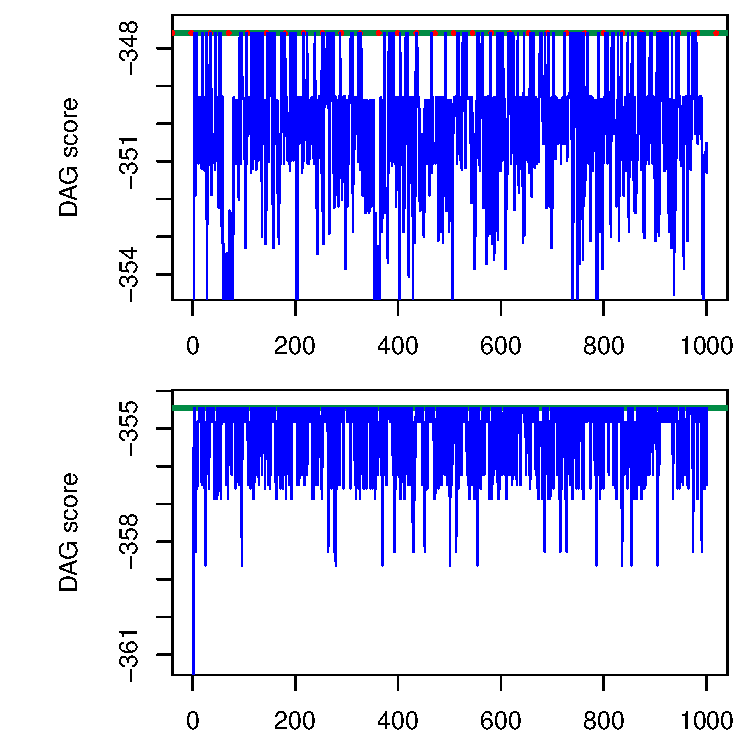
\includegraphics[width=\maxwidth]{figure/minimal-unnamed-chunk-15-1} 

}



\end{knitrout}

\section{New edge reversal move}

We can include the new edge reversal move, by simply making the vector \texttt{moveprobs} have two elements, with the second corresponding to the probability of picking the new edge reversal move.

\begin{knitrout}
\definecolor{shadecolor}{rgb}{0.969, 0.969, 0.969}\color{fgcolor}\begin{kframe}
\begin{alltt}
\hlstd{moveprobs} \hlkwb{<-} \hlkwd{c}\hlstd{(}\hlnum{0.93}\hlstd{,} \hlnum{0.07}\hlstd{)}  \hlcom{# having length 1 disallows the new edge reversal move}
\end{alltt}
\end{kframe}
\end{knitrout}

\nn Now we run the chains for 40000 iterations, once with the standard edge reversal and once without

\begin{knitrout}
\definecolor{shadecolor}{rgb}{0.969, 0.969, 0.969}\color{fgcolor}\begin{kframe}
\begin{alltt}
\hlstd{iterations} \hlkwb{<-} \hlnum{40000}  \hlcom{#number of iterations in the chain}
\hlstd{stepsave} \hlkwb{<-} \hlstd{iterations}\hlopt{/}\hlnum{1000}  \hlcom{#how often to save the result}
\hlstd{revallowed} \hlkwb{<-} \hlnum{1}  \hlcom{# allow standard edge reversals}
\hlkwd{set.seed}\hlstd{(seednumber)}  \hlcom{# set the seed}
\hlstd{example} \hlkwb{<-} \hlkwd{structureMCMC}\hlstd{(n, startDAG, iterations, stepsave, maxparents,}
    \hlstd{parenttable, scoretable, revallowed, moveprobs)}  \hlcom{# run the MCMC code}
\hlstd{revallowed} \hlkwb{<-} \hlnum{0}  \hlcom{# don't allow standard edge reversals}
\hlkwd{set.seed}\hlstd{(seednumber)}
\hlstd{example2} \hlkwb{<-} \hlkwd{structureMCMC}\hlstd{(n, startDAG, iterations, stepsave, maxparents,}
    \hlstd{parenttable, scoretable, revallowed, moveprobs)}
\end{alltt}
\end{kframe}
\end{knitrout}

\nn The trace plot is now

\begin{knitrout}
\definecolor{shadecolor}{rgb}{0.969, 0.969, 0.969}\color{fgcolor}\begin{kframe}
\begin{alltt}
\hlkwd{par}\hlstd{(}\hlkwc{mfrow} \hlstd{=} \hlkwd{c}\hlstd{(}\hlnum{2}\hlstd{,} \hlnum{1}\hlstd{))}  \hlcom{# plotting parameters}
\hlkwd{par}\hlstd{(}\hlkwc{mar} \hlstd{=} \hlkwd{c}\hlstd{(}\hlnum{2.5}\hlstd{,} \hlnum{5.75}\hlstd{,} \hlnum{0.5}\hlstd{,} \hlnum{0.75}\hlstd{))}

\hlstd{nparts} \hlkwb{<-} \hlkwd{length}\hlstd{(example[[}\hlnum{2}\hlstd{]])}
\hlstd{maxDAGscore} \hlkwb{<-} \hlkwd{max}\hlstd{(}\hlkwd{unlist}\hlstd{(example[[}\hlnum{2}\hlstd{]]))}

\hlkwd{plot}\hlstd{(}\hlnum{1}\hlopt{:}\hlstd{nparts, example[[}\hlnum{2}\hlstd{]],} \hlkwc{type} \hlstd{=} \hlstr{"l"}\hlstd{,} \hlkwc{ylab} \hlstd{=} \hlstr{"DAG score"}\hlstd{,} \hlkwc{xlab} \hlstd{=} \hlstr{""}\hlstd{,}
    \hlkwc{main} \hlstd{=} \hlstr{""}\hlstd{,} \hlkwc{col} \hlstd{=} \hlstr{"blue"}\hlstd{,} \hlkwc{ylim} \hlstd{=} \hlkwd{c}\hlstd{(maxDAGscore} \hlopt{-} \hlnum{6.8}\hlstd{, maxDAGscore} \hlopt{+}
        \hlnum{0.2}\hlstd{))}
\hlkwd{abline}\hlstd{(}\hlkwc{h} \hlstd{= maxDAGscore,} \hlkwc{col} \hlstd{=} \hlstr{"springgreen4"}\hlstd{,} \hlkwc{lwd} \hlstd{=} \hlnum{3}\hlstd{)}
\hlkwd{abline}\hlstd{(}\hlkwc{h} \hlstd{= realDAGlogscore,} \hlkwc{col} \hlstd{=} \hlstr{"red"}\hlstd{,} \hlkwc{lty} \hlstd{=} \hlnum{3}\hlstd{,} \hlkwc{lwd} \hlstd{=} \hlnum{3}\hlstd{)}
\hlkwd{lines}\hlstd{(}\hlnum{1}\hlopt{:}\hlstd{nparts, example[[}\hlnum{2}\hlstd{]],} \hlkwc{type} \hlstd{=} \hlstr{"l"}\hlstd{,} \hlkwc{col} \hlstd{=} \hlstr{"blue"}\hlstd{)}

\hlstd{maxDAGscore2} \hlkwb{<-} \hlkwd{max}\hlstd{(}\hlkwd{unlist}\hlstd{(example2[[}\hlnum{2}\hlstd{]]))}

\hlkwd{plot}\hlstd{(}\hlnum{1}\hlopt{:}\hlstd{nparts, example2[[}\hlnum{2}\hlstd{]],} \hlkwc{type} \hlstd{=} \hlstr{"l"}\hlstd{,} \hlkwc{ylab} \hlstd{=} \hlstr{"DAG score"}\hlstd{,} \hlkwc{xlab} \hlstd{=} \hlstr{""}\hlstd{,}
    \hlkwc{main} \hlstd{=} \hlstr{""}\hlstd{,} \hlkwc{col} \hlstd{=} \hlstr{"blue"}\hlstd{,} \hlkwc{ylim} \hlstd{=} \hlkwd{c}\hlstd{(maxDAGscore2} \hlopt{-} \hlnum{6.8}\hlstd{, maxDAGscore2} \hlopt{+}
        \hlnum{0.2}\hlstd{))}
\hlkwd{abline}\hlstd{(}\hlkwc{h} \hlstd{= maxDAGscore2,} \hlkwc{col} \hlstd{=} \hlstr{"springgreen4"}\hlstd{,} \hlkwc{lwd} \hlstd{=} \hlnum{3}\hlstd{)}
\hlkwd{abline}\hlstd{(}\hlkwc{h} \hlstd{= realDAGlogscore,} \hlkwc{col} \hlstd{=} \hlstr{"red"}\hlstd{,} \hlkwc{lty} \hlstd{=} \hlnum{3}\hlstd{,} \hlkwc{lwd} \hlstd{=} \hlnum{3}\hlstd{)}
\hlkwd{lines}\hlstd{(}\hlnum{1}\hlopt{:}\hlstd{nparts, example2[[}\hlnum{2}\hlstd{]],} \hlkwc{type} \hlstd{=} \hlstr{"l"}\hlstd{,} \hlkwc{col} \hlstd{=} \hlstr{"blue"}\hlstd{)}
\end{alltt}
\end{kframe}

{\centering 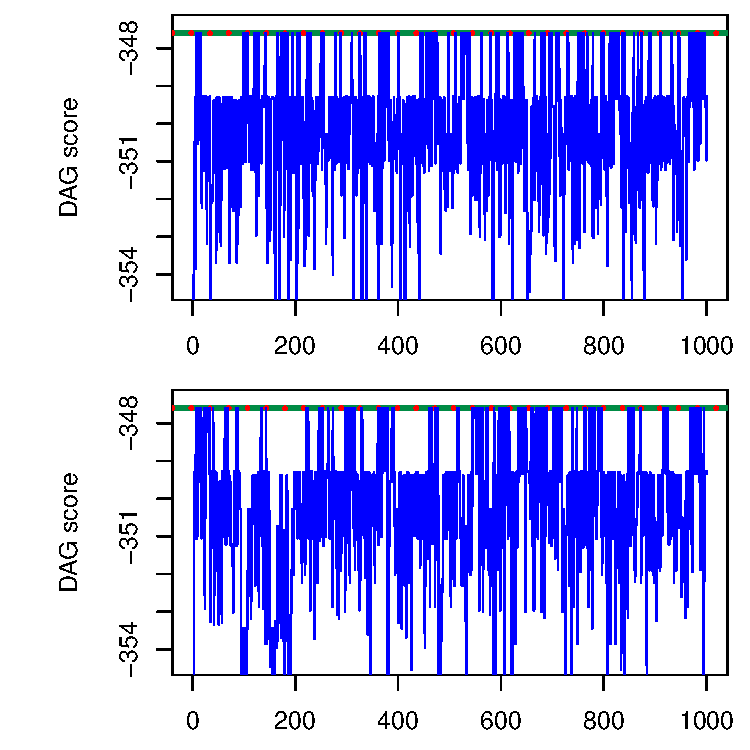
\includegraphics[width=\maxwidth]{figure/minimal-unnamed-chunk-18-1} 

}



\end{knitrout}

\section{Order MCMC}

\nn For Order MCMC we now have three elements in the \texttt{moveprobs} vector.  The first is the probability of swapping any two elements in the order, the second the probability of only swapping adjacent nodes and the last the probability to stay still (to enforce aperiodicity of the chain)

\begin{knitrout}
\definecolor{shadecolor}{rgb}{0.969, 0.969, 0.969}\color{fgcolor}\begin{kframe}
\begin{alltt}
\hlstd{prob1} \hlkwb{<-} \hlnum{99}
\hlkwa{if} \hlstd{(n} \hlopt{>} \hlnum{3}\hlstd{) \{}
    \hlstd{prob1} \hlkwb{<-} \hlkwd{round}\hlstd{(}\hlnum{6} \hlopt{*} \hlnum{99} \hlopt{*} \hlstd{n}\hlopt{/}\hlstd{(n}\hlopt{^}\hlnum{2} \hlopt{+} \hlnum{10} \hlopt{*} \hlstd{n} \hlopt{-} \hlnum{24}\hlstd{))}
\hlstd{\}}
\hlstd{prob1} \hlkwb{<-} \hlstd{prob1}\hlopt{/}\hlnum{100}
\hlstd{moveprobs} \hlkwb{<-} \hlkwd{c}\hlstd{(prob1,} \hlnum{0.99} \hlopt{-} \hlstd{prob1,} \hlnum{0.01}\hlstd{)}
\hlstd{moveprobs} \hlkwb{<-} \hlstd{moveprobs}\hlopt{/}\hlkwd{sum}\hlstd{(moveprobs)}  \hlcom{# normalisation}
\hlstd{moveprobs}
\end{alltt}
\begin{verbatim}
[1] 0.58 0.41 0.01
\end{verbatim}
\end{kframe}
\end{knitrout}

\nn We also need to choose a starting order, for example the identity permutation

\begin{knitrout}
\definecolor{shadecolor}{rgb}{0.969, 0.969, 0.969}\color{fgcolor}\begin{kframe}
\begin{alltt}
\hlstd{startorder} \hlkwb{<-} \hlkwd{c}\hlstd{(}\hlnum{1}\hlopt{:}\hlstd{n)}  \hlcom{# starting order}
\end{alltt}
\end{kframe}
\end{knitrout}

\nn and then we can run the MCMC code for 20000 iterations

\begin{knitrout}
\definecolor{shadecolor}{rgb}{0.969, 0.969, 0.969}\color{fgcolor}\begin{kframe}
\begin{alltt}
\hlstd{iterations} \hlkwb{<-} \hlnum{20000}  \hlcom{#number of iterations in the chain}
\hlstd{stepsave} \hlkwb{<-} \hlstd{iterations}\hlopt{/}\hlnum{1000}  \hlcom{#how often to save the result}
\hlkwd{set.seed}\hlstd{(seednumber)}  \hlcom{# set the seed}
\hlstd{example} \hlkwb{<-} \hlkwd{orderMCMC}\hlstd{(n, startorder, iterations, stepsave, parenttable,}
    \hlstd{scoretable, moveprobs)}
\end{alltt}
\end{kframe}
\end{knitrout}

\nn The output now contains four components, a sampled DAG and its score along with the score of the entire order and the sampled order itself (stored as a permutation vector).  We can plot the outcome for both the orders and for the DAGs

\begin{knitrout}
\definecolor{shadecolor}{rgb}{0.969, 0.969, 0.969}\color{fgcolor}\begin{kframe}
\begin{alltt}
\hlkwd{par}\hlstd{(}\hlkwc{mfrow} \hlstd{=} \hlkwd{c}\hlstd{(}\hlnum{2}\hlstd{,} \hlnum{1}\hlstd{))}  \hlcom{# plotting parameters}
\hlkwd{par}\hlstd{(}\hlkwc{mar} \hlstd{=} \hlkwd{c}\hlstd{(}\hlnum{2.5}\hlstd{,} \hlnum{5.75}\hlstd{,} \hlnum{0.5}\hlstd{,} \hlnum{0.75}\hlstd{))}

\hlstd{nparts} \hlkwb{<-} \hlkwd{length}\hlstd{(example[[}\hlnum{2}\hlstd{]])}
\hlstd{maxorderscore} \hlkwb{<-} \hlkwd{max}\hlstd{(}\hlkwd{unlist}\hlstd{(example[[}\hlnum{3}\hlstd{]]))}
\hlstd{maxDAGscore} \hlkwb{<-} \hlkwd{max}\hlstd{(}\hlkwd{unlist}\hlstd{(example[[}\hlnum{2}\hlstd{]]))}

\hlkwd{plot}\hlstd{(}\hlnum{1}\hlopt{:}\hlstd{nparts, example[[}\hlnum{3}\hlstd{]],} \hlkwc{type} \hlstd{=} \hlstr{"l"}\hlstd{,} \hlkwc{ylab} \hlstd{=} \hlstr{"Order score"}\hlstd{,}
    \hlkwc{xlab} \hlstd{=} \hlstr{""}\hlstd{,} \hlkwc{main} \hlstd{=} \hlstr{""}\hlstd{,} \hlkwc{col} \hlstd{=} \hlstr{"blue"}\hlstd{,} \hlkwc{ylim} \hlstd{=} \hlkwd{c}\hlstd{(maxorderscore} \hlopt{-}
        \hlnum{6.8}\hlstd{, maxorderscore} \hlopt{+} \hlnum{0.2}\hlstd{))}
\hlkwd{abline}\hlstd{(}\hlkwc{h} \hlstd{= maxorderscore,} \hlkwc{col} \hlstd{=} \hlstr{"springgreen4"}\hlstd{,} \hlkwc{lwd} \hlstd{=} \hlnum{3}\hlstd{)}
\hlkwd{abline}\hlstd{(}\hlkwc{h} \hlstd{= realorderlogscores,} \hlkwc{col} \hlstd{=} \hlstr{"red"}\hlstd{,} \hlkwc{lty} \hlstd{=} \hlnum{3}\hlstd{,} \hlkwc{lwd} \hlstd{=} \hlnum{3}\hlstd{)}
\hlkwd{lines}\hlstd{(}\hlnum{1}\hlopt{:}\hlstd{nparts, example[[}\hlnum{3}\hlstd{]],} \hlkwc{type} \hlstd{=} \hlstr{"l"}\hlstd{,} \hlkwc{col} \hlstd{=} \hlstr{"blue"}\hlstd{)}

\hlkwd{plot}\hlstd{(}\hlnum{1}\hlopt{:}\hlstd{nparts, example[[}\hlnum{2}\hlstd{]],} \hlkwc{type} \hlstd{=} \hlstr{"l"}\hlstd{,} \hlkwc{ylab} \hlstd{=} \hlstr{"DAG score"}\hlstd{,} \hlkwc{xlab} \hlstd{=} \hlstr{""}\hlstd{,}
    \hlkwc{main} \hlstd{=} \hlstr{""}\hlstd{,} \hlkwc{col} \hlstd{=} \hlstr{"blue"}\hlstd{,} \hlkwc{ylim} \hlstd{=} \hlkwd{c}\hlstd{(maxDAGscore} \hlopt{-} \hlnum{6.8}\hlstd{, maxDAGscore} \hlopt{+}
        \hlnum{0.2}\hlstd{))}
\hlkwd{abline}\hlstd{(}\hlkwc{h} \hlstd{= maxDAGscore,} \hlkwc{col} \hlstd{=} \hlstr{"springgreen4"}\hlstd{,} \hlkwc{lwd} \hlstd{=} \hlnum{3}\hlstd{)}
\hlkwd{abline}\hlstd{(}\hlkwc{h} \hlstd{= realDAGlogscore,} \hlkwc{col} \hlstd{=} \hlstr{"red"}\hlstd{,} \hlkwc{lty} \hlstd{=} \hlnum{3}\hlstd{,} \hlkwc{lwd} \hlstd{=} \hlnum{3}\hlstd{)}
\hlkwd{lines}\hlstd{(}\hlnum{1}\hlopt{:}\hlstd{nparts, example[[}\hlnum{2}\hlstd{]],} \hlkwc{type} \hlstd{=} \hlstr{"l"}\hlstd{,} \hlkwc{col} \hlstd{=} \hlstr{"blue"}\hlstd{)}
\end{alltt}
\end{kframe}

{\centering 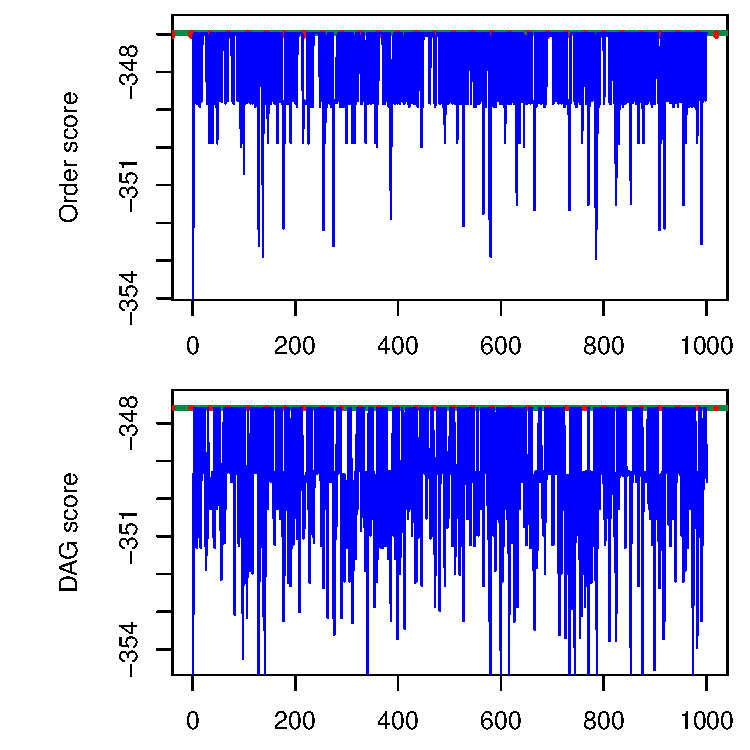
\includegraphics[width=\maxwidth]{figure/minimal-unnamed-chunk-22-1} 

}



\end{knitrout}

\section{Partition MCMC}

\nn For Partiton MCMC we have five elements in the \texttt{moveprobs} vector.  The first is the probability of swapping two nodes from different partititon elements, while the second for swapping nodes from adjacent partition elements.  The third corresponds to joining and splitting partition elements with the fourth being the probability of moving a node from one element to another.  The last is again the probability of not moving

\begin{knitrout}
\definecolor{shadecolor}{rgb}{0.969, 0.969, 0.969}\color{fgcolor}\begin{kframe}
\begin{alltt}
\hlstd{prob1start} \hlkwb{<-} \hlnum{40}\hlopt{/}\hlnum{100}
\hlstd{prob1} \hlkwb{<-} \hlstd{prob1start} \hlopt{*} \hlnum{100}
\hlkwa{if} \hlstd{(n} \hlopt{>} \hlnum{3}\hlstd{) \{}
    \hlstd{prob1} \hlkwb{<-} \hlkwd{round}\hlstd{(}\hlnum{6} \hlopt{*} \hlstd{prob1} \hlopt{*} \hlstd{n}\hlopt{/}\hlstd{(n}\hlopt{^}\hlnum{2} \hlopt{+} \hlnum{10} \hlopt{*} \hlstd{n} \hlopt{-} \hlnum{24}\hlstd{))}
\hlstd{\}}
\hlstd{prob1} \hlkwb{<-} \hlstd{prob1}\hlopt{/}\hlnum{100}
\hlstd{prob2start} \hlkwb{<-} \hlnum{99}\hlopt{/}\hlnum{100} \hlopt{-} \hlstd{prob1start}
\hlstd{prob2} \hlkwb{<-} \hlstd{prob2start} \hlopt{*} \hlnum{100}
\hlkwa{if} \hlstd{(n} \hlopt{>} \hlnum{3}\hlstd{) \{}
    \hlstd{prob2} \hlkwb{<-} \hlkwd{round}\hlstd{(}\hlnum{6} \hlopt{*} \hlstd{prob2} \hlopt{*} \hlstd{n}\hlopt{/}\hlstd{(n}\hlopt{^}\hlnum{2} \hlopt{+} \hlnum{10} \hlopt{*} \hlstd{n} \hlopt{-} \hlnum{24}\hlstd{))}
\hlstd{\}}
\hlstd{prob2} \hlkwb{<-} \hlstd{prob2}\hlopt{/}\hlnum{100}
\hlstd{moveprobs} \hlkwb{<-} \hlkwd{c}\hlstd{(prob1, prob1start} \hlopt{-} \hlstd{prob1, prob2start} \hlopt{-} \hlstd{prob2, prob2,}
    \hlnum{0.01}\hlstd{)}
\hlstd{moveprobs} \hlkwb{<-} \hlstd{moveprobs}\hlopt{/}\hlkwd{sum}\hlstd{(moveprobs)}  \hlcom{# normalisation}
\hlstd{moveprobs}
\end{alltt}
\begin{verbatim}
[1] 0.24 0.16 0.24 0.35 0.01
\end{verbatim}
\end{kframe}
\end{knitrout}

\nn For the starting partition we can choose the DAG with no edges

\begin{knitrout}
\definecolor{shadecolor}{rgb}{0.969, 0.969, 0.969}\color{fgcolor}\begin{kframe}
\begin{alltt}
\hlstd{startpermutation} \hlkwb{<-} \hlkwd{c}\hlstd{(}\hlnum{1}\hlopt{:}\hlstd{n)}  \hlcom{# pick a starting permutation}
\hlstd{startpartition} \hlkwb{<-} \hlkwd{c}\hlstd{(n)}  \hlcom{# and a starting partition - c(n) gives the empty DAG}
\end{alltt}
\end{kframe}
\end{knitrout}

\nn and then run the MCMC code for 10000 iterations

\begin{knitrout}
\definecolor{shadecolor}{rgb}{0.969, 0.969, 0.969}\color{fgcolor}\begin{kframe}
\begin{alltt}
\hlstd{iterations} \hlkwb{<-} \hlnum{10000}  \hlcom{#number of iterations in the chain}
\hlstd{stepsave} \hlkwb{<-} \hlstd{iterations}\hlopt{/}\hlnum{1000}  \hlcom{#how often to save the result}
\hlkwd{set.seed}\hlstd{(seednumber)}  \hlcom{# set the seed}
\hlstd{example} \hlkwb{<-} \hlkwd{partitionMCMC}\hlstd{(n, startpermutation, startpartition, iterations,}
    \hlstd{stepsave, parenttable, scoretable, moveprobs)}
\end{alltt}
\end{kframe}
\end{knitrout}

\nn The output now contains a five components: a sampled DAG and its score, the score of the entire partition and the sampled permutation and partition.  The trace plot is

\begin{knitrout}
\definecolor{shadecolor}{rgb}{0.969, 0.969, 0.969}\color{fgcolor}\begin{kframe}
\begin{alltt}
\hlkwd{par}\hlstd{(}\hlkwc{mfrow} \hlstd{=} \hlkwd{c}\hlstd{(}\hlnum{2}\hlstd{,} \hlnum{1}\hlstd{))}  \hlcom{# plotting parameters}
\hlkwd{par}\hlstd{(}\hlkwc{mar} \hlstd{=} \hlkwd{c}\hlstd{(}\hlnum{2.5}\hlstd{,} \hlnum{5.75}\hlstd{,} \hlnum{0.5}\hlstd{,} \hlnum{0.75}\hlstd{))}

\hlstd{nparts} \hlkwb{<-} \hlkwd{length}\hlstd{(example[[}\hlnum{2}\hlstd{]])}
\hlstd{maxpartitionscore} \hlkwb{<-} \hlkwd{max}\hlstd{(}\hlkwd{unlist}\hlstd{(example[[}\hlnum{3}\hlstd{]]))}
\hlstd{maxDAGscore} \hlkwb{<-} \hlkwd{max}\hlstd{(}\hlkwd{unlist}\hlstd{(example[[}\hlnum{2}\hlstd{]]))}

\hlkwd{plot}\hlstd{(}\hlnum{1}\hlopt{:}\hlstd{nparts, example[[}\hlnum{3}\hlstd{]],} \hlkwc{type} \hlstd{=} \hlstr{"l"}\hlstd{,} \hlkwc{ylab} \hlstd{=} \hlstr{"Partition score"}\hlstd{,}
    \hlkwc{xlab} \hlstd{=} \hlstr{""}\hlstd{,} \hlkwc{main} \hlstd{=} \hlstr{""}\hlstd{,} \hlkwc{col} \hlstd{=} \hlstr{"blue"}\hlstd{,} \hlkwc{ylim} \hlstd{=} \hlkwd{c}\hlstd{(maxpartitionscore} \hlopt{-}
        \hlnum{6.8}\hlstd{, maxpartitionscore} \hlopt{+} \hlnum{0.2}\hlstd{))}
\hlkwd{abline}\hlstd{(}\hlkwc{h} \hlstd{= maxpartitionscore,} \hlkwc{col} \hlstd{=} \hlstr{"springgreen4"}\hlstd{,} \hlkwc{lwd} \hlstd{=} \hlnum{3}\hlstd{)}
\hlkwd{abline}\hlstd{(}\hlkwc{h} \hlstd{= realpartitionlogscore,} \hlkwc{col} \hlstd{=} \hlstr{"red"}\hlstd{,} \hlkwc{lty} \hlstd{=} \hlnum{3}\hlstd{,} \hlkwc{lwd} \hlstd{=} \hlnum{3}\hlstd{)}
\hlkwd{lines}\hlstd{(}\hlnum{1}\hlopt{:}\hlstd{nparts, example[[}\hlnum{3}\hlstd{]],} \hlkwc{type} \hlstd{=} \hlstr{"l"}\hlstd{,} \hlkwc{col} \hlstd{=} \hlstr{"blue"}\hlstd{)}

\hlkwd{plot}\hlstd{(}\hlnum{1}\hlopt{:}\hlstd{nparts, example[[}\hlnum{2}\hlstd{]],} \hlkwc{type} \hlstd{=} \hlstr{"l"}\hlstd{,} \hlkwc{ylab} \hlstd{=} \hlstr{"DAG score"}\hlstd{,} \hlkwc{xlab} \hlstd{=} \hlstr{""}\hlstd{,}
    \hlkwc{main} \hlstd{=} \hlstr{""}\hlstd{,} \hlkwc{col} \hlstd{=} \hlstr{"blue"}\hlstd{,} \hlkwc{ylim} \hlstd{=} \hlkwd{c}\hlstd{(maxDAGscore} \hlopt{-} \hlnum{6.8}\hlstd{, maxDAGscore} \hlopt{+}
        \hlnum{0.2}\hlstd{))}
\hlkwd{abline}\hlstd{(}\hlkwc{h} \hlstd{= maxDAGscore,} \hlkwc{col} \hlstd{=} \hlstr{"springgreen4"}\hlstd{,} \hlkwc{lwd} \hlstd{=} \hlnum{3}\hlstd{)}
\hlkwd{abline}\hlstd{(}\hlkwc{h} \hlstd{= realDAGlogscore,} \hlkwc{col} \hlstd{=} \hlstr{"red"}\hlstd{,} \hlkwc{lty} \hlstd{=} \hlnum{3}\hlstd{,} \hlkwc{lwd} \hlstd{=} \hlnum{3}\hlstd{)}
\hlkwd{lines}\hlstd{(}\hlnum{1}\hlopt{:}\hlstd{nparts, example[[}\hlnum{2}\hlstd{]],} \hlkwc{type} \hlstd{=} \hlstr{"l"}\hlstd{,} \hlkwc{col} \hlstd{=} \hlstr{"blue"}\hlstd{)}
\end{alltt}
\end{kframe}

{\centering 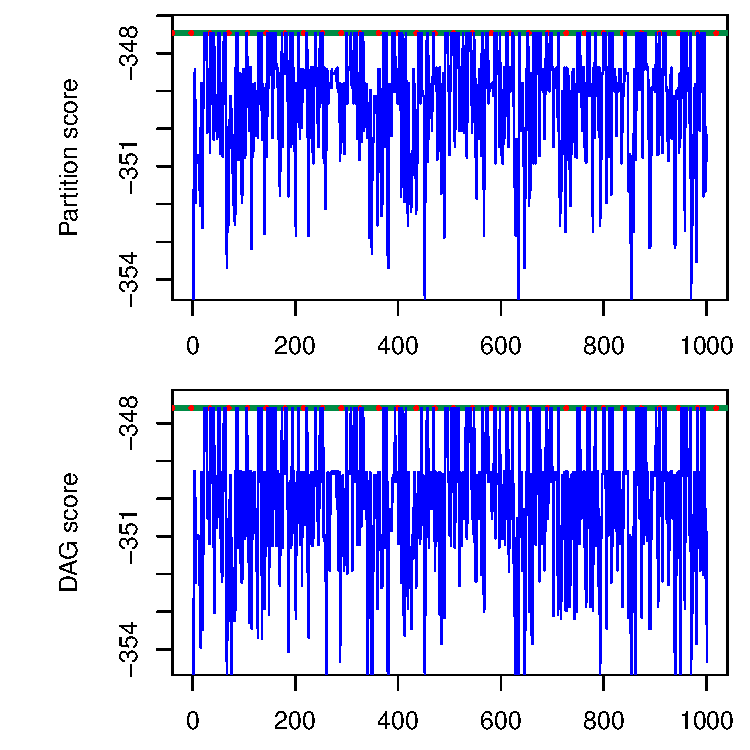
\includegraphics[width=\maxwidth]{figure/minimal-unnamed-chunk-26-1} 

}



\end{knitrout}

\section{Partition MCMC with edge reversal}

\nn Finally we can include the new edge reversal move on an underlying Partition MCMC chain by including a sixth element in the \texttt{moveprobs} vector, corresponding to the probability of picking the edge reversal move

\begin{knitrout}
\definecolor{shadecolor}{rgb}{0.969, 0.969, 0.969}\color{fgcolor}\begin{kframe}
\begin{alltt}
\hlstd{prob1start} \hlkwb{<-} \hlnum{37}\hlopt{/}\hlnum{100}
\hlstd{prob1} \hlkwb{<-} \hlstd{prob1start} \hlopt{*} \hlnum{100}
\hlkwa{if} \hlstd{(n} \hlopt{>} \hlnum{3}\hlstd{) \{}
    \hlstd{prob1} \hlkwb{<-} \hlkwd{round}\hlstd{(}\hlnum{6} \hlopt{*} \hlstd{prob1} \hlopt{*} \hlstd{n}\hlopt{/}\hlstd{(n}\hlopt{^}\hlnum{2} \hlopt{+} \hlnum{10} \hlopt{*} \hlstd{n} \hlopt{-} \hlnum{24}\hlstd{))}
\hlstd{\}}
\hlstd{prob1} \hlkwb{<-} \hlstd{prob1}\hlopt{/}\hlnum{100}
\hlstd{prob2start} \hlkwb{<-} \hlnum{92}\hlopt{/}\hlnum{100} \hlopt{-} \hlstd{prob1start}
\hlstd{prob2} \hlkwb{<-} \hlstd{prob2start} \hlopt{*} \hlnum{100}
\hlkwa{if} \hlstd{(n} \hlopt{>} \hlnum{3}\hlstd{) \{}
    \hlstd{prob2} \hlkwb{<-} \hlkwd{round}\hlstd{(}\hlnum{6} \hlopt{*} \hlstd{prob2} \hlopt{*} \hlstd{n}\hlopt{/}\hlstd{(n}\hlopt{^}\hlnum{2} \hlopt{+} \hlnum{10} \hlopt{*} \hlstd{n} \hlopt{-} \hlnum{24}\hlstd{))}
\hlstd{\}}
\hlstd{prob2} \hlkwb{<-} \hlstd{prob2}\hlopt{/}\hlnum{100}
\hlstd{moveprobs} \hlkwb{<-} \hlkwd{c}\hlstd{(prob1, prob1start} \hlopt{-} \hlstd{prob1, prob2start} \hlopt{-} \hlstd{prob2, prob2,}
    \hlnum{0.01}\hlstd{,} \hlnum{0.07}\hlstd{)}
\hlstd{moveprobs} \hlkwb{<-} \hlstd{moveprobs}\hlopt{/}\hlkwd{sum}\hlstd{(moveprobs)}  \hlcom{# normalisation}
\hlstd{moveprobs}
\end{alltt}
\begin{verbatim}
[1] 0.22 0.15 0.23 0.32 0.01 0.07
\end{verbatim}
\end{kframe}
\end{knitrout}

\nn This we run for 9000 iterations

\begin{knitrout}
\definecolor{shadecolor}{rgb}{0.969, 0.969, 0.969}\color{fgcolor}\begin{kframe}
\begin{alltt}
\hlstd{iterations} \hlkwb{<-} \hlnum{9000}  \hlcom{#number of iterations in the chain}
\hlstd{stepsave} \hlkwb{<-} \hlstd{iterations}\hlopt{/}\hlnum{1000}  \hlcom{#how often to save the result}
\hlkwd{set.seed}\hlstd{(seednumber)}  \hlcom{# set the seed}
\hlstd{example} \hlkwb{<-} \hlkwd{partitionMCMC}\hlstd{(n, startpermutation, startpartition, iterations,}
    \hlstd{stepsave, parenttable, scoretable, moveprobs)}
\end{alltt}
\end{kframe}
\end{knitrout}

\nn and plot the results

\begin{knitrout}
\definecolor{shadecolor}{rgb}{0.969, 0.969, 0.969}\color{fgcolor}\begin{kframe}
\begin{alltt}
\hlkwd{par}\hlstd{(}\hlkwc{mfrow} \hlstd{=} \hlkwd{c}\hlstd{(}\hlnum{2}\hlstd{,} \hlnum{1}\hlstd{))}  \hlcom{# plotting parameters}
\hlkwd{par}\hlstd{(}\hlkwc{mar} \hlstd{=} \hlkwd{c}\hlstd{(}\hlnum{2.5}\hlstd{,} \hlnum{5.75}\hlstd{,} \hlnum{0.5}\hlstd{,} \hlnum{0.75}\hlstd{))}

\hlstd{nparts} \hlkwb{<-} \hlkwd{length}\hlstd{(example[[}\hlnum{2}\hlstd{]])}
\hlstd{maxpartitionscore} \hlkwb{<-} \hlkwd{max}\hlstd{(}\hlkwd{unlist}\hlstd{(example[[}\hlnum{3}\hlstd{]]))}
\hlstd{maxDAGscore} \hlkwb{<-} \hlkwd{max}\hlstd{(}\hlkwd{unlist}\hlstd{(example[[}\hlnum{2}\hlstd{]]))}

\hlkwd{plot}\hlstd{(}\hlnum{1}\hlopt{:}\hlstd{nparts, example[[}\hlnum{3}\hlstd{]],} \hlkwc{type} \hlstd{=} \hlstr{"l"}\hlstd{,} \hlkwc{ylab} \hlstd{=} \hlstr{"Partition score"}\hlstd{,}
    \hlkwc{xlab} \hlstd{=} \hlstr{""}\hlstd{,} \hlkwc{main} \hlstd{=} \hlstr{""}\hlstd{,} \hlkwc{col} \hlstd{=} \hlstr{"blue"}\hlstd{,} \hlkwc{ylim} \hlstd{=} \hlkwd{c}\hlstd{(maxpartitionscore} \hlopt{-}
        \hlnum{6.8}\hlstd{, maxpartitionscore} \hlopt{+} \hlnum{0.2}\hlstd{))}
\hlkwd{abline}\hlstd{(}\hlkwc{h} \hlstd{= maxpartitionscore,} \hlkwc{col} \hlstd{=} \hlstr{"springgreen4"}\hlstd{,} \hlkwc{lwd} \hlstd{=} \hlnum{3}\hlstd{)}
\hlkwd{abline}\hlstd{(}\hlkwc{h} \hlstd{= realpartitionlogscore,} \hlkwc{col} \hlstd{=} \hlstr{"red"}\hlstd{,} \hlkwc{lty} \hlstd{=} \hlnum{3}\hlstd{,} \hlkwc{lwd} \hlstd{=} \hlnum{3}\hlstd{)}
\hlkwd{lines}\hlstd{(}\hlnum{1}\hlopt{:}\hlstd{nparts, example[[}\hlnum{3}\hlstd{]],} \hlkwc{type} \hlstd{=} \hlstr{"l"}\hlstd{,} \hlkwc{col} \hlstd{=} \hlstr{"blue"}\hlstd{)}

\hlkwd{plot}\hlstd{(}\hlnum{1}\hlopt{:}\hlstd{nparts, example[[}\hlnum{2}\hlstd{]],} \hlkwc{type} \hlstd{=} \hlstr{"l"}\hlstd{,} \hlkwc{ylab} \hlstd{=} \hlstr{"DAG score"}\hlstd{,} \hlkwc{xlab} \hlstd{=} \hlstr{""}\hlstd{,}
    \hlkwc{main} \hlstd{=} \hlstr{""}\hlstd{,} \hlkwc{col} \hlstd{=} \hlstr{"blue"}\hlstd{,} \hlkwc{ylim} \hlstd{=} \hlkwd{c}\hlstd{(maxDAGscore} \hlopt{-} \hlnum{6.8}\hlstd{, maxDAGscore} \hlopt{+}
        \hlnum{0.2}\hlstd{))}
\hlkwd{abline}\hlstd{(}\hlkwc{h} \hlstd{= maxDAGscore,} \hlkwc{col} \hlstd{=} \hlstr{"springgreen4"}\hlstd{,} \hlkwc{lwd} \hlstd{=} \hlnum{3}\hlstd{)}
\hlkwd{abline}\hlstd{(}\hlkwc{h} \hlstd{= realDAGlogscore,} \hlkwc{col} \hlstd{=} \hlstr{"red"}\hlstd{,} \hlkwc{lty} \hlstd{=} \hlnum{3}\hlstd{,} \hlkwc{lwd} \hlstd{=} \hlnum{3}\hlstd{)}
\hlkwd{lines}\hlstd{(}\hlnum{1}\hlopt{:}\hlstd{nparts, example[[}\hlnum{2}\hlstd{]],} \hlkwc{type} \hlstd{=} \hlstr{"l"}\hlstd{,} \hlkwc{col} \hlstd{=} \hlstr{"blue"}\hlstd{)}
\end{alltt}
\end{kframe}

{\centering 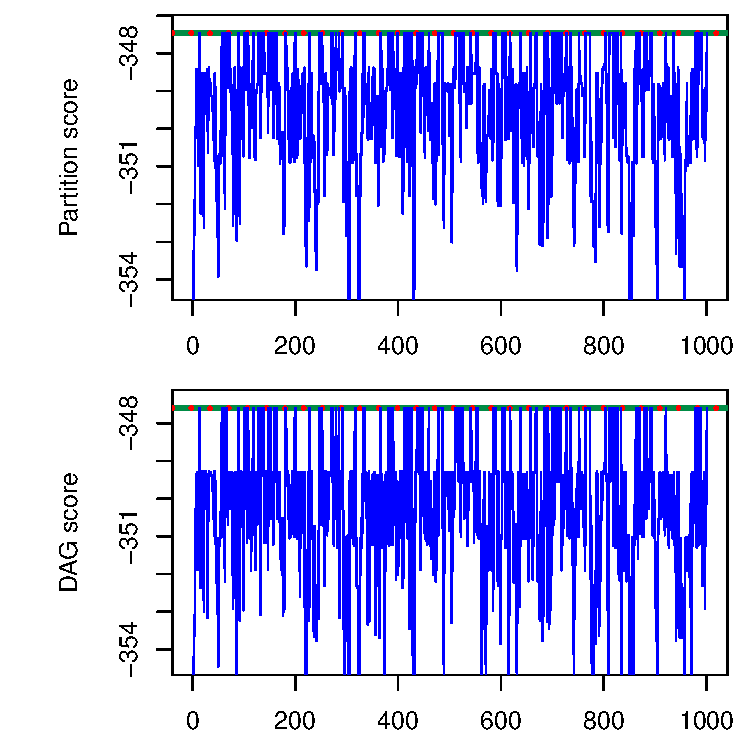
\includegraphics[width=\maxwidth]{figure/minimal-unnamed-chunk-29-1} 

}



\end{knitrout}

\end{document}
